\documentclass[a4paper,11pt,UKenglish,twoside,openright]{report}\usepackage[]{graphicx}\usepackage[]{color}
% maxwidth is the original width if it is less than linewidth
% otherwise use linewidth (to make sure the graphics do not exceed the margin)
\makeatletter
\def\maxwidth{ %
  \ifdim\Gin@nat@width>\linewidth
    \linewidth
  \else
    \Gin@nat@width
  \fi
}
\makeatother

\usepackage{Sweavel}



\usepackage{uiothesis}

\title{Identifying School Climate Variables Associated with Students' Financial Literacy Outcomes}
\subtitle{A Cross-Country Comparison\\Using {PISA} 2018 Data}
\author{Tony C. A. Tan}

\begin{document}

% Input faculty etc info
\duoforside[
    fac={Faculty of Educational Sciences},
    dept={Centre for Educational Measurement},
    program={Assessment, Measurement and Evaluation},
    date={Spring 2021},
%  printer={X-press printing house},
    short
]

% Change page numbering to roman
\pagenumbering{roman}

% Create an acknowledgement page
\thispagestyle{empty}

% This is where I generated the Chinese characters
%//ref http://www.akuziti.com/mb/
% I used font 24.Huawen Xingkai and 100 pixel
\vspace*{\fill}
\begin{figure*}[h]
    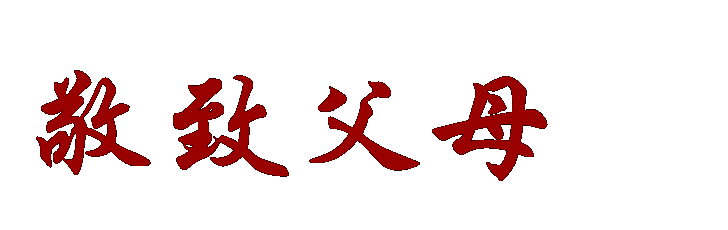
\includegraphics[width=\textwidth]{./Figures/To-parents.png}
\end{figure*}
\begin{flushright}
To my parents
\end{flushright}
\vspace*{\fill}
%\newpage
\clearpage
\thispagestyle{empty}

\vspace*{3cm}

\begin{quote}
    \calligra\huge      % Changes the font to caligraphy and huge size.
\hyphenchar\font=-1     % Stops LaTeX from splitting/hyphenating words
Study hard what interests you the most in the most undisciplined, irreverent and original manner possible.
\end{quote}

\begin{figure*}[h]
    \flushright
    
\includegraphics[width=0.50\textwidth]{./Figures/Feynman-Signature.jpg}
\end{figure*}
\vspace*{-1cm}

%\begin{flushright}
%--- Richard P. Feynman
%\end{flushright}

\setcounter{page}{0}
% End of acknowledgement page

% Put Table of Content here
\tableofcontents

% Put a List of Tables here
\listoftables

% Put a List of Figures here
\listoffigures



% APA7 Rule 2.21 Line Spacing
%\onehalfspacing
\doublespacing

% Acknowledgement

\chapter*{Acknowledgement}
\label{Ack}



% Popular Abstract

\chapter*{Popular Abstract}
\label{Ab.0}



% Abstract

\chapter*{Abstract}
\label{Ab.1}


% End of front matter. None of the pages so far counts towards the page limit.
\clearpage
\thispagestyle{empty}

% Restart page number. Page count starts here.
\pagenumbering{arabic}
\setcounter{page}{0} % Do not swap these two command. Need new chapter to be "Open right".

% Chapter 1 Introduction
%<<child="Chapters/Ch1.Rnw", tidy=FALSE, message=FALSE, warning=FALSE>>=
%@

% Chapter 2 Theoretical framework
%<<child="Chapters/Ch2.Rnw", tidy=FALSE, message=FALSE, warning=FALSE>>=
%@

% Chapter 3 Methods

\chapter{Methods}
\label{chp:3}

\section{Model Equations}

\newpage

Student-Level ($L_1$):

\begin{equation}
    \begin{aligned}
        \texttt{LEISURE}_{ij} &= \alpha_{0j}^{M_1} + \gamma_{11}\texttt{ESCS}_{ij} + \gamma_{21}\texttt{FEMALE}_{ij} + r^{M_1}_{ij}\\
        \texttt{SCHWK}_{ij} &= \alpha_{0j}^{M_2} + \gamma_{12}\texttt{ESCS}_{ij} + \gamma_{22}\texttt{FEMALE}_{ij} + r^{M_3}_{ij}\\
        \texttt{USESCH}_{ij} &= \alpha_{0j}^{M_3} + \gamma_{13}\texttt{ESCS}_{ij} + \gamma_{23}\texttt{FEMALE}_{ij} + r^{M_4}_{ij}\\
        \texttt{READJOY}_{ij}  &= \alpha_{0j}^{M_4} + \beta_{14}\texttt{LEISURE}_{ij} + \beta_{24}\texttt{SCHWK}_{ij} + \beta_{34}\texttt{USESCH}_{ij} + \gamma_{34}\texttt{IMMI1} + \gamma_{44}\texttt{IMMI2}_{ij} + r^{M_4}_{ij}\\
        \texttt{READCOMP}_{ij} &= \alpha_{0j}^{M_5} \beta_{15}\texttt{LEISURE}_{ij} + \beta_{25}\texttt{SCHWK}_{ij} +  \beta_{35}\texttt{USESCH}_{ij} + \gamma_{35}\texttt{IMMI1}_{ij} + \gamma_{45}\texttt{IMMI2}_{ij} + r^{M_5}_{ij}\\
        \texttt{READEASE}_{ij} &= \alpha_{0j}^{M_6} + \beta_{16}\texttt{LEISURE}_{ij} + \beta_{26}\texttt{SCHWK}_{ij} +  \beta_{36}\texttt{USESCH}_{ij} + \gamma_{36}\texttt{IMMI1}_{ij} + \gamma_{46}\texttt{IMMI2}_{ij} + r^{M_6}_{ij}\\
        \texttt{READ}_{ij} &= \alpha_{0j}^{M_7} + \beta_{17}\texttt{LEISURE}_{ij} + \beta_{27}\texttt{SCHWK}_{ij} + \beta_{37}\texttt{USESCH}_{ij}\\
        &+ \beta_{47}\texttt{READJOY}_{ij} + \beta_{57}\texttt{READCOMP}_{ij} + \beta_{67}\texttt{READEASE}_{ij} + r^{M_7}_{ij}
    \end{aligned}
\end{equation}

School-Level ($L_2$):

\begin{equation}
    \alpha_{0j}^{M_7} = \alpha_{00} + a_1\texttt{LEISURE}_j + a_2\texttt{SCHWK}_j + a_3\texttt{USESCH}_j + a_4\texttt{POLICY}_j + \epsilon_j
\end{equation}

\newpage


\begin{equation}
    \begin{aligned}
        \text{Student-Level ($L_1$):}\\
        \begin{bmatrix}
            \texttt{LEISURE}_{ij}\\
            \texttt{SCHWK}_{ij}\\
            \texttt{USESCH}_{ij}\\
            \texttt{READJOY}_{ij}\\
            \texttt{READCOMP}_{ij}\\
            \texttt{READEASE}_{ij}\\
            \texttt{READ}_{ij}
        \end{bmatrix} &=
        \begin{pmatrix}
            \alpha_{0j}^{M_1}\\
            \alpha_{0j}^{M_2}\\
            \alpha_{0j}^{M_3}\\
            \alpha_{0j}^{M_4}\\
            \alpha_{0j}^{M_5}\\
            \alpha_{0j}^{M_6}\\
            \alpha_{0j}^{M_7}
        \end{pmatrix} +
        \begin{pmatrix}
            0   &0  &0  &\beta_{14}   &\beta_{15}  &\beta_{16}   &\beta_{17}\\
            0   &0  &0  &\beta_{24}   &\beta_{25}  &\beta_{26}   &\beta_{27}\\
            0   &0  &0  &\beta_{34}   &\beta_{35}  &\beta_{36}   &\beta_{37}\\
            0   &0  &0  &0            &0           &0            &\beta_{47}\\
            0   &0  &0  &0            &0           &0            &\beta_{57}\\
            0   &0  &0  &0            &0           &0            &\beta_{67}\\
            0   &0  &0  &0            &0           &0            &0\\
        \end{pmatrix}\Ts
        \begin{bmatrix}
            \texttt{LEISURE}_{ij}\\
            \texttt{SCHWK}_{ij}\\
            \texttt{USESCH}_{ij}\\
            \texttt{READJOY}_{ij}\\
            \texttt{READCOMP}_{ij}\\
            \texttt{READEASE}_{ij}\\
            \texttt{READ}_{ij}
        \end{bmatrix}\\
        &+
        \begin{pmatrix}
            \gamma_{11}  &\gamma_{12}   &\gamma_{13}    &0  &0   &0   &0\\
            \gamma_{21}  &\gamma_{22}   &\gamma_{23}    &0  &0   &0   &0\\
            0   &0   &0  &\gamma_{34}   &\gamma_{35}    &\gamma_{36}  &0\\
            0   &0   &0  &\gamma_{44}   &\gamma_{45}    &\gamma_{46}  &0
        \end{pmatrix}\Ts
        \begin{bmatrix}
            \texttt{ESCS}_{ij}\\
            \texttt{FEMALE}_{ij}\\
            \texttt{IMMI1GEN}_{ij}\\
            \texttt{IMMI2GEN}_{ij}
        \end{bmatrix} +
        \begin{pmatrix}
            r^{M_1}_{ij}\\
            r^{M_2}_{ij}\\
            r^{M_3}_{ij}\\
            r^{M_4}_{ij}\\
            r^{M_5}_{ij}\\
            r^{M_6}_{ij}\\
            r^{M_7}_{ij}
        \end{pmatrix}\\
        \text{School-Level ($L_2$):}\\
        \alpha^{M_7}_{0j} &= \alpha_{00} +
        \begin{pmatrix}
            a_1\\
            a_2\\
            a_3\\
            a_4
        \end{pmatrix}\Ts
        \begin{bmatrix}
            \texttt{LEISURE}_j\\
            \texttt{SCHWK}_j\\
            \texttt{USESCH}_j\\
            \texttt{POLICY}_j
        \end{bmatrix}
        + \epsilon_j
    \end{aligned}
\end{equation}

% Chapter 4 Results
%<<child="Chapters/Ch4.Rnw", tidy=FALSE, message=FALSE, warning=FALSE>>=
%@

% Chapter 5 Discussion
%<<child="Chapters/Ch5.Rnw", tidy=FALSE, message=FALSE, warning=FALSE>>=
%@

% Put Reference here
\newpage
\printbibliography[title=References]

% New CEMO policy: leave tables and figures close to the paragraphs that discussed them.

% Tables
%\newpage
%<<child="Tables/tab.Rnw", tidy=FALSE, message=FALSE, warning=FALSE>>=
%@

% Figures
%\newpage
%<<child="Figures/fig.Rnw", tidy=FALSE, message=FALSE, warning=FALSE>>=
%@

%\newpage

% Insert appendices
\begin{appendices}
    \begin{singlespace}
%    \chapter[GDPR Documentation and Ethical Approval]{GDPR Documentation and\\Ethical Approval} % Square brackets is for TOC. Curly brackets for actual page.

%\epigraph{\flushleft --- Do you know a good \textsc{GDPR} consultant?\\ --- Yes.\\ --- Can you pass me their email address?\\ --- No.}

This research project discharges its duty imposed by the \textsc{EEA}'s general data protection regulation (\textsc{GDPR}) by following Norwegian Centre for Research Data (\textsc{NSD})'s \href{https://nsd.no/personvernombud/en/notify/notification_test.html}{notification test} on Friday, 11 September 2020. Both \href{https://www.oecd.org/pisa/data/2018database/}{\textsc{PISA} 2018 Database} and the \href{https://data.worldbank.org/}{World Bank Open Data} contain only aggregated and de-personalised datasets with no possibility of back-tracing to any particular participant. Resultantly, no identifiable personal data were collected or used at any stage of this research. The \textsc{NSD}'s assessment letter outlines the agency's decision of not subjecting this project to the \textsc{GDPR} notification. The \textsc{NSD} decision letter also satisfies University of Oslo's \href{https://www.uio.no/english/for-employees/support/research/funding/units/hf/imv/data-ethics/}{ethical approval requirement} and concludes the approval process.

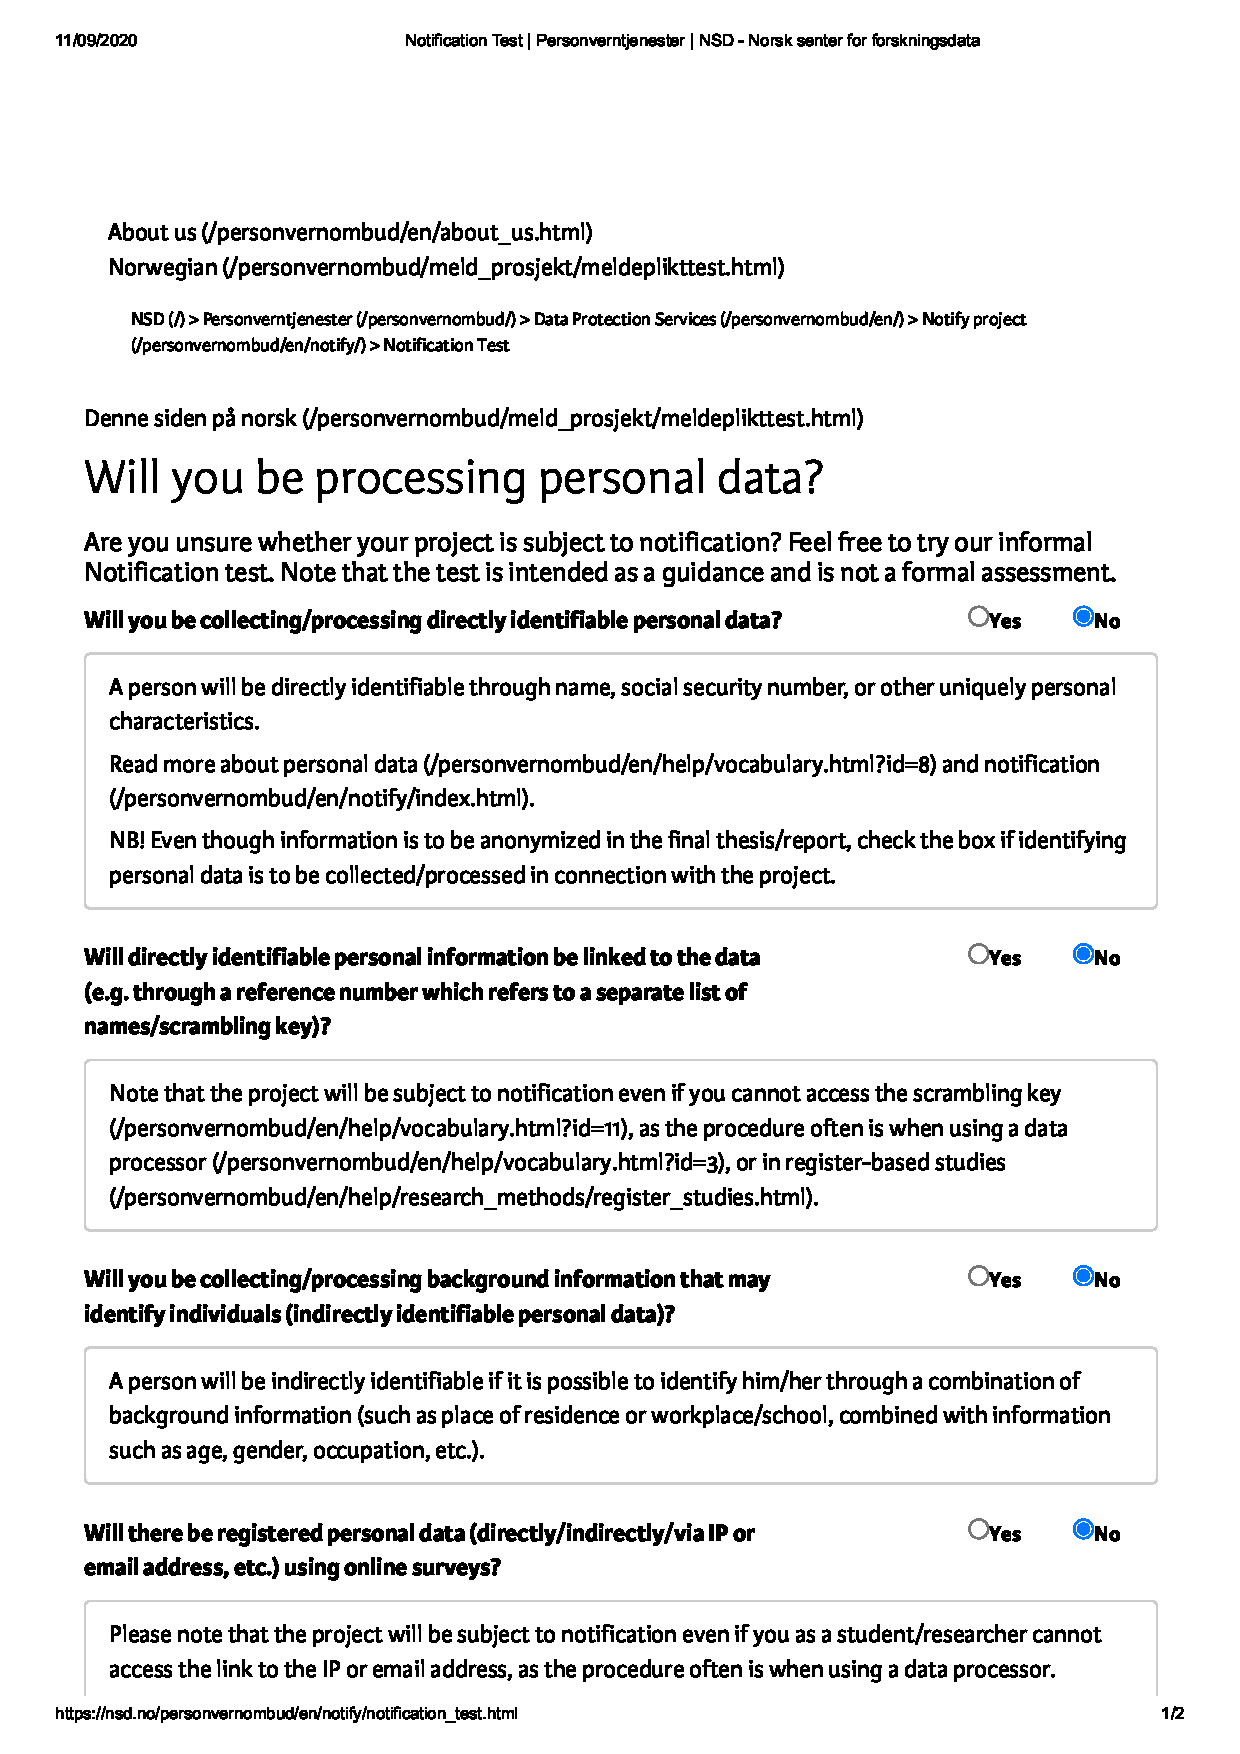
\includepdf[pages=-,fitpaper=true,noautoscale=true]{Appendices/Notification-Test.pdf}

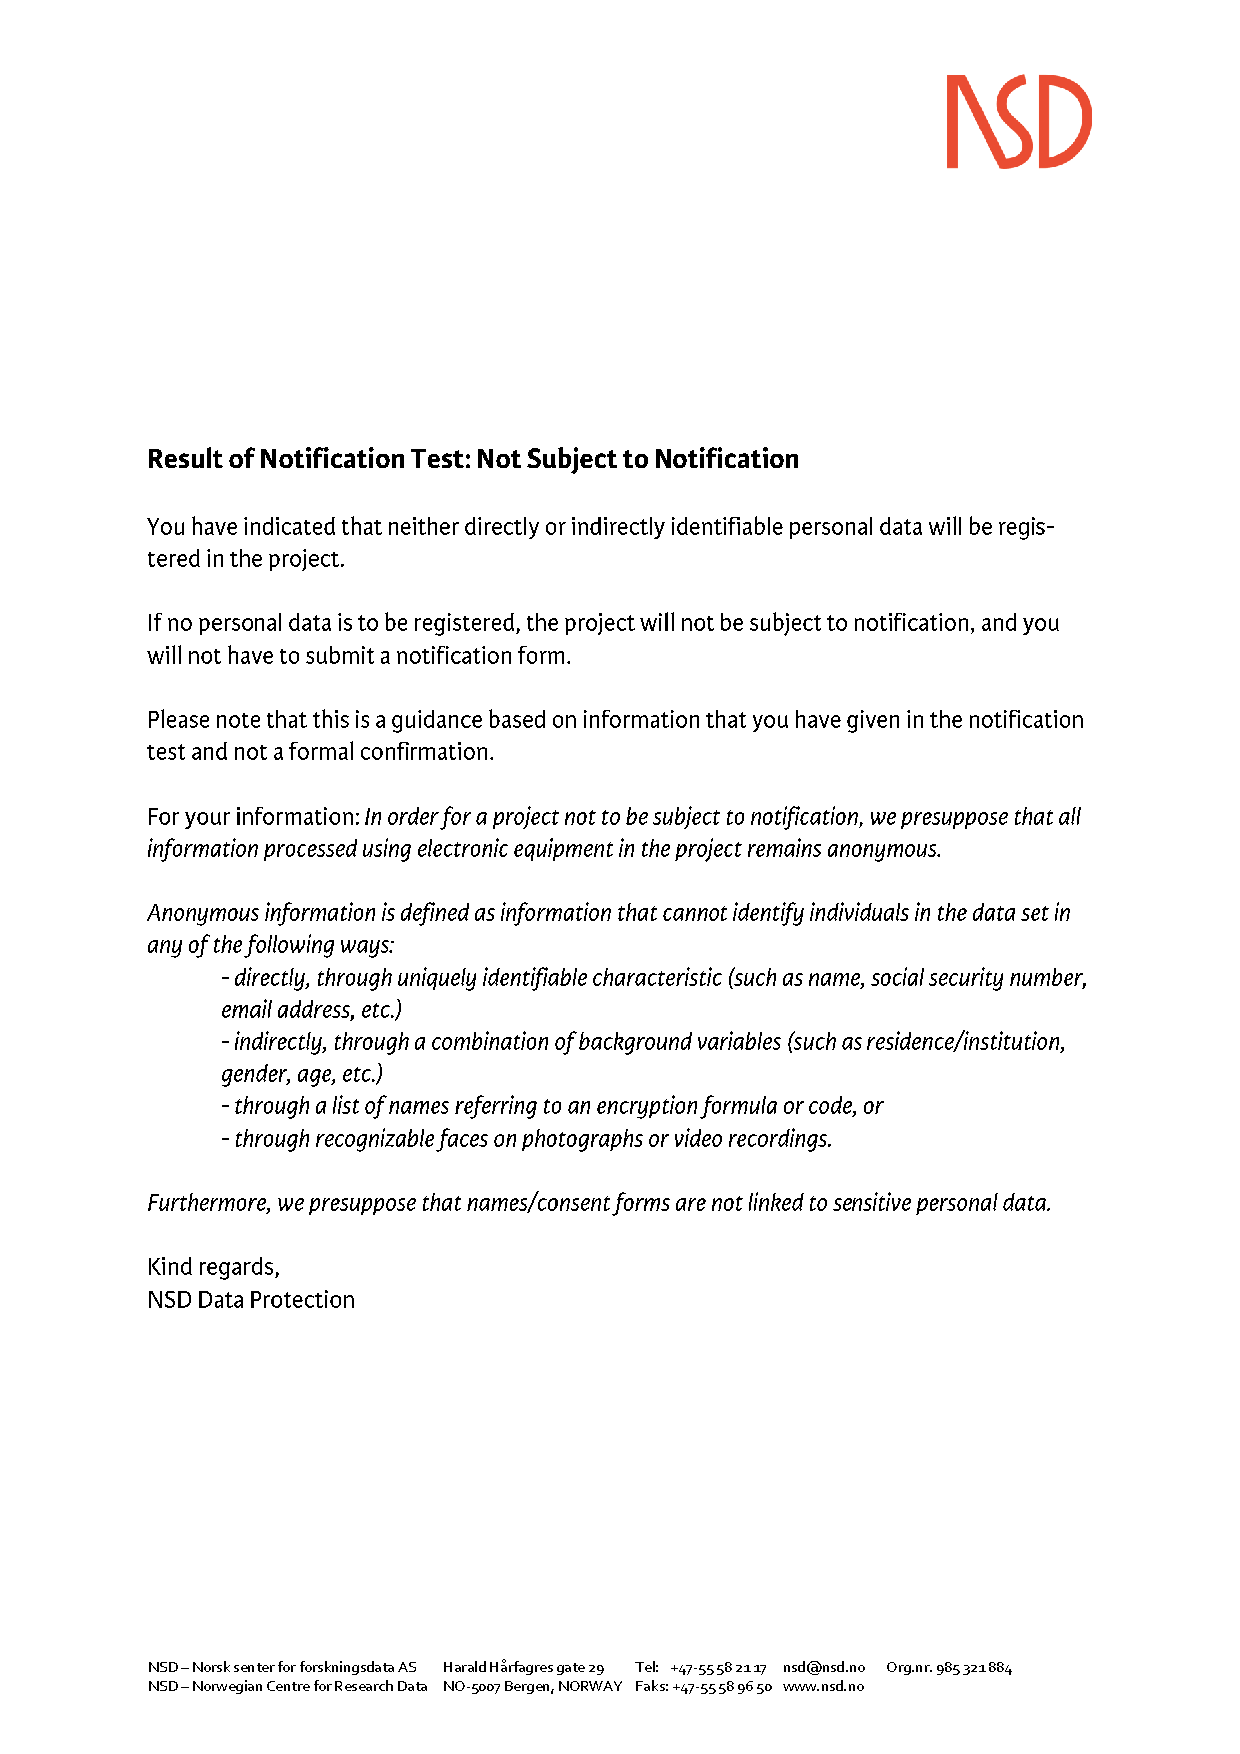
\includepdf[pages=-,fitpaper=true,noautoscale=true]{Appendices/not_subject_to_notification.pdf}


%    %\setcounter{secnumdepth}{0}
\chapter{Analysis Code}

\begin{singlespace}

\section{Chapter 1}

There is no analysis code in \cref{chp:1}.

\section{Chapter 2}

\subsection{Data Import} \label{R.import} \footnotesize
\lstinputlisting[language=R,style=vscodeR]{./R/0 Import.R}

\subsection{Missing Pattern Inspection} \label{R.missing} \footnotesize
\lstinputlisting[language=R,style=vscodeR]{./R/1 Missing.R}

\subsection{Financial Knowledge Index} \label{R.fki} \footnotesize
\lstinputlisting[language=R,style=vscodeR]{./R/2 FKI.R}

\subsection{Data Reimport} \label{R.reimport} \footnotesize
\lstinputlisting[language=R,style=vscodeR]{./R/3 Reimport.R}

\end{singlespace}

%    \chapter{Derivation of Country-level Financial Knowledge Indices}

%\epigraph{There are two things you are better off not watching in the making: sausages and\\ econometric estimates.}{Edward Leamer}

\section{Theoretical Foundation}

PISA 2018 financial literacy dataset \parencite{FLdata} provides rich information about students and schools. For the purpose of cross-country comparison, however, the country-level data must be addressed separately by the researchers. \textcite{morenoherrero:2018a}, for instance, introduced a variable ``quality of math and science education'' to control for country-level differences since consensus is yet to emerge about the most appropriate measure for ``countries' financial knowledge''. Inspired by the UN's approach to forming Human Development Indices, a recent publication \textcite{olivermarquez:2020} highlighted four aspects of countries' macroeconomic practices in their attempt to develop country-level financial knowledge indices (FKI).

Oliver-M{\'a}rquez and colleagues consider a country's economic capability, represented by its GDP per capita, to be a key dimension in bringing about its FKI. Secondly, literature converges on the importance of education training for a country's financial knowledge capability \parencite{oecd:2005}. Thirdly, countries with regular engagement with sophisticated financial products and financial markets should possess higher FKI. Lastly, countries with higher aggregate consumption levels and with ageing populations are likely to possess higher FKI due to more frequent exposure and pressure in retirement provision, respetively.

More specifically, \textcite{olivermarquez:2020} suggests using the logarithm of GDP per capital in current international dollars (purchasing power parity adjusted) as a measure for the \texttt{Economic Capability} sub-index. For the \texttt{Education Training} sub-index, the authors consider postgraduate-to-total-tertiary-graduation ratios as a reflection of ``highly skilled'' workforce and the mean years of schooling as a measure of countries' general education levels. For the \texttt{Use} sub-index, gross portfolio equity assets (GPEA) and insurance company assets (ICA) are considered sophisticated financial products countries engage themselves in. Additionally, in order to capture the central role of technology in amplifying the proliferation and use of financial assets, the proportion of Internet users (\textsc{IUS}) enters the definition via
\[ \texttt{Use} = ( \text{GPEA} + \text{ICA} ) ^ \text{IUS}. \]
For the final sub-index \texttt{Need}, the authors define
\[ \texttt{Need} = ( \text{PFA} + \text{AC} ) ^ \text{AGEING}, \]
where \textsc{PFA} is the pension-fund-assets-to-\textsc{GDP} ratio. Aggregate consumption is defined as:
\[ \text{AC} = \frac{2\% \times \text{household final consumption expenditure}}{\text{GDP}}, \]
where the ``$2\%$ rule'' is drawn from \textcite{caliendo:2013} and the proportion of ageing population is computed as
\[ \text{AGEING} = \frac{ \left[ \frac{\text{population}(>65)}{\text{population}(20 \sim 64)} \right]_{2018} - \left[ \frac{\text{population}(>65)}{\text{population}(20 \sim 64)} \right]_{2009} }{ \left[ \frac{\text{population}(>65)}{\text{population}(20 \sim 64)} \right]_{2009} }. \]

\section{Data Collection and Missing Data Treatment}

The data sources for FKI computation are documented in \cref{tab:FKIsource} and its associated notes. The sub-indices \texttt{Educational Training} and \texttt{Use} both contain missing observations for the year 2018. Majority of such missing data appear to be the result of administrative delay, with historic observations available until 2017. It is therefore feasible to conduct time-series forecasts using prior year observations to best approximate 2018 values.

\ltable{tab:FKIsource}{Data Sources for FKI Computation}{
    \begin{tabular}{cclc}
    \toprule
    \multicolumn{1}{c}{Database$\ ^\text{a}$} & Country$\ ^\text{b}$ & \multicolumn{1}{c}{Series} & Time \\
    \midrule
    \rowcolor[rgb]{ .9,  .9,  .9} \multicolumn{4}{c}{Economic Capacity} \\
    WB-dev & 20    & GDP per capita, PPP (current international \$) & 2018 \\
    \rowcolor[rgb]{ .9,  .9,  .9} \multicolumn{4}{c}{Educational Training} \\
    WB-ed & 20 \textbackslash\ Russia & Graduates from ISCED 7 programmes in tertiary education, both sexes (number) & 2013--\textbf{2018} \\
          &       & Graduates from ISCED 8 programmes in tertiary education, both sexes (number) & 2013--\textbf{2018} \\
          &       & Graduates from tertiary education, both sexes (number) & 2013--\textbf{2018} \\
    RS & Russia & PhD (Type 1)$\ ^\text{c}$, PhD (Type 2)$\ ^\text{d}$ & 2018 \\
    RE & Russia & Master (Type 1)$\ ^\text{e}$, Master (Type 2)$\ ^\text{f}$, total tertiary \emph{excluding} PhD$\ ^\text{g}$ & 2018 \\
    HDR & 20    & Dimension = Education; Education = Mean years of schooling (years) & 2018 \\
    \rowcolor[rgb]{ .9,  .9,  .9} \multicolumn{4}{c}{Use} \\
    WB-fin & 20    & Gross portfolio equity assets to GDP (\%) & 2011--\textbf{2018} \\
           &       & Insurance company assets to GDP (\%) & 2011--\textbf{2018} \\
    WB-dev & 20    & Individuals using the Internet (\% of population) & 2009--\textbf{2018} \\
    \rowcolor[rgb]{ .9,  .9,  .9} \multicolumn{4}{c}{Need} \\
    WB-fin & 20 \textbackslash\ Georgia & Pension fund assets to GDP (\%) & 2008--\textbf{2018} \\
    GP & Georgia & Minutes of the meeting of the investment board of the Pension Agency$\ ^\text{h}$ & $\textcolor{white}{\ ^\text{*}}$2019$\ ^\text{*}$ \\
    GS & Georgia & GDP at current prices, billion GEL$\ ^\text{i}$ & 2018 \\
    WB-dev & 20    & Household and NPISHs final consumption expenditure, PPP (current international \$) & 2018 \\
          &       & GDP, PPP (current international \$) & 2018 \\
          &       & Population ages 0--14, male & 2009, 2018 \\
          &       & Population ages 0--14, female & 2009, 2018 \\
          &       & Population ages 15--64, male & 2009, 2018 \\
          &       & Population ages 15--64, female & 2009, 2018 \\
          &       & Population ages 65 and above, male & 2009, 2018 \\
          &       & Population ages 65 and above, female & 2009, 2018 \\
          &       & Population ages 15--19, male (\% of male population) & 2009, 2018 \\
          &       & Population ages 15--19, female (\% of female population) & 2009, 2018 \\
          \bottomrule
    \end{tabular}
}{Sub-indices are shaded in gray. Bold font signifies this year contains missing data.}{3}
\newpage

\begin{singlespace} \small
\begin{itemize}
    \item[$^\text{a}$] WB-dev = \href{https://databank.worldbank.org/source/world-development-indicators}{World Bank -- World development indicators}\\
        WB-ed = \href{https://databank.worldbank.org/source/education-statistics-^-all-indicators}{World Bank -- Education statistics -- All indicators}\\
        WB-fin = \href{https://databank.worldbank.org/source/global-financial-development}{World Bank -- Global financial development}\\
        HDR = \href{http://hdr.undp.org/en/data}{Human Development Reports -- Data}\\
        RS = \href{https://rosstat.gov.ru/}{Russian Federal State Statistic Service}\\
        RE = \href{https://minobrnauki.gov.ru}{Russian Ministry of Education and Science}\\
        GP = \href{https://www.pensions.ge}{Pension Agency of Georgia}\\
        GS = \href{https://www.geostat.ge}{National Statistics Office of Georgia}
    \item[$^\text{b}$] ``20'' = the 20 participating countries in 2018 \textsc{PISA} financial literacy test: Brazil, Bulgaria, Canada, Chile, Estonia, Finland, Georgia, Indonesia, Italy, Latvia, Lithuania, the Netherlands, Peru, Poland, Portugal, Russian Federation, Serbia, Slovak Republic, Spain, and the USA. ``\textbackslash'' = exluding or except
    \item[$^\text{c}$] \href{https://rosstat.gov.ru/storage/mediabank/asp-2(1).xls}{https://rosstat.gov.ru/storage/mediabank/asp-2(1).xls}, Sheet ``\foreignlanguage{russian}{по направлениям подготовки}'', Cell C7 = number of PhD graduates \mbox{(Type 1)}
    \item[$^\text{d}$] \href{https://rosstat.gov.ru/storage/mediabank/asp-3.xls}{https://rosstat.gov.ru/storage/mediabank/asp-3.xls}, Sheet ``\foreignlanguage{russian}{по научным специальностям}'', Cell B7 = number of PhD graduates \mbox{(Type 2)}
    \item[$^\text{e--g}$] \href{https://minobrnauki.gov.ru/common/upload/download/VPO_1_2018.rar}{https://minobrnauki.gov.ru/common/upload/download/VPO{\textunderscore}1{\textunderscore}2018.rar} contains a spreadsheet \textcolor{blue}{\foreignlanguage{russian}{СВОД{\textunderscore}ВПО1{\textunderscore}ВСЕГО}.xls}, Sheet ``P2{\textunderscore}1{\textunderscore}3(1)'', Cell E198 = number of master graduates (Type 1)$^\text{e}$, Cell E410 = number of master graduates (Type 2)$^\text{f}$, Cell E592 = total tertiary graduates \emph{excluding} PhD$^\text{g}$
    \item[$^\text{h}$] \href{https://www.pensions.ge/docs/legislation/investment-board-protocol-4.pdf}{Minutes of the meeting of the investment board of the Pension Agency}, p. 4, no. 3
    \item[$^\text{i}$] \href{https://www.geostat.ge/en/modules/categories/23/gross-domestic-product-gdp}{Gross domestic product (GDP)}, row = GDP at current prices, billion GEL, column = 2018
    \item[$^\text{*}$] Georgia started a \href{https://agenda.ge/en/news/2019/13}{new pension system} on 1 January 2019. Since 2018 was a transitional period with scarce data, 2019 is used as the best approximation for Georgia's pension system for 2018.
\end{itemize}
\end{singlespace}

\clearpage



\subsection{Sub-index \texttt{Educational Training}}

The 2018 archive for the number of master (ISCED 7), PhD (ISCED 8), and total tertiary graduates are incomplete for all participating countries except Georgia, Indonesia and Serbia. \cref{fig:skilled} presents a time series plot of
\[ \texttt{highly skilled} = \frac{\text{number of masters} + \text{number of PhDs}}{\text{total number of tertiary graduates}} \]
and suggests that this ratio is likely to be stable over time, especially between adjacent years. A ``naive forecast'', where the nearest available year's data are to be duplicated for 2018, is applied for \texttt{highly skilled}.

\pfigure{fig:skilled}{Proportion of Postgraduates to Total Tertiary Graduations}{1}{./Figures/skilled.pdf}{``Postgraduate'' is defined as master (ISCED 7) and PhD (ISCED 8) graduates. Countries not shown: GEO, IDN and SRB (2018 data available) and RUS (consult other sources)}{1.75}{1.25}

\subsection{Sub-index \texttt{Use}}

All series involved in calculating this sub-index, GPEA, ICA and IUS, contain missing data. When time series data contain only exponential growth but no underlying trend, a simple exponential smoothing would suffice \parencite{garder:1985}; if trend is present, Holt-Winters method is superior \parencite{chatfield:1978}. \cref{fig:use} facilitates this decision making by plotting both the original and log-transformed versions of GPEA and ICA series. Since curves after log-transformations have slopes, it is prudent to apply the Holt-Winters forecasting method in order to account for possible trends contained in the original series.

\pfigure{fig:use}{Time Series Trend Test}{1}{./Figures/use.pdf}{The time series plots after natural logarithm transformations (bottom panels) are not flat, suggesting the original series (top panels) contain trends. Holt-Winters method therefore is preferred over simple exponential smoothing for 2018 forecasts.}{0.5}{0.85}

The IUS series contains missing data for Canada, Chile and the United States. Similar Holt-Winters procedure is applied to recover 2018 IUS data.

\ltable{tab:FKIraw}{Data Utilised for Computing FKI}{
  \begin{tabular}{cd{3} c d{3}d{1} c d{3}d{3}d{3} c d{3}d{3}d{3}}
    \toprule
    & \multicolumn{1}{c}{Economic Capacity} &       & \multicolumn{2}{c}{Educational Training} &       & \multicolumn{3}{c}{Use} &       & \multicolumn{3}{c}{Need} \\
\cmidrule{2-2}\cmidrule{4-5}\cmidrule{7-9}\cmidrule{11-13}          & \multicolumn{1}{c}{GDP per capita} &       & \multicolumn{1}{c}{Skilled} & \multicolumn{1}{c}{Schooling} &       & \multicolumn{1}{c}{GPEA} & \multicolumn{1}{c}{ICA} & \multicolumn{1}{c}{IUS} &       & \multicolumn{1}{c}{PFA} & \multicolumn{1}{c}{AC} & \multicolumn{1}{c}{AGEING} \\
    \midrule
    BRA   & 9.612 &       & 6.484 & 7.8   &       & 1.683 & 16.259 & 70.434 &       & 11.827 & 1.210  & 0.288 \\
    BGR   & 10.026 &       & 45.294 & 11.8  &       & 4.114 & 7.044 & 64.782 &       & 13.577 & 1.091 & 0.234 \\
    CAN   & 10.821 &       & 15.832 & 13.3  &       & 84.010 & 77.728 & 93.588 &       & 96.205 & 1.068 & 0.271 \\
    CHL   & 10.117 &       & 16.371 & 10.4  &       & 51.755 & 25.591 & 89.531 &       & 73.225 & 1.073 & 0.214 \\
    EST   & 10.501 &       & 36.765 & 13.0  &       & 16.399 & 7.681 & 89.357 &       & 18.012 & 0.876 & 0.163 \\
    FIN   & 10.807 &       & 35.024 & 12.4  &       & 93.626 & 31.481 & 88.890 &       & 52.024 & 0.974 & 0.370 \\
    GEO   & 9.588 &       & 24.039 & 12.8  &       & 0.784 & 1.469 & 62.718 &       & 0.834 & 1.227 & 0.042 \\
    IDN   & 9.362 &       & 7.771 & 8.0   &       & 0.636 & 4.612 & 39.905 &       & 1.826 & 1.059 & 0.145 \\
    ITA   & 10.665 &       & 44.771 & 10.2  &       & 57.434 & 51.260 & 74.387 &       & 10.589 & 1.075 & 0.155 \\
    LVA   & 10.330 &       & 29.554 & 12.8  &       & 8.598 & 2.538 & 83.577 &       & 14.732 & 1.027 & 0.142 \\
    LTU   & 10.487 &       & 28.749 & 13.0  &       & 9.008 & 5.500 & 79.723 &       & 7.457 & 1.107 & 0.149 \\
    NLD   & 10.961 &       & 32.590 & 12.2  &       & 124.171 & 64.956 & 94.712 &       & 207.938 & 0.805 & 0.326 \\
    PER   & 9.479 &       & 13.577 & 9.2   &       & 16.027 & 6.505 & 52.540 &       & 22.530 & 1.187 & 0.227 \\
    POL   & 10.368 &       & 36.725 & 12.3  &       & 4.853 & 9.535 & 77.542 &       & 9.838 & 1.085 & 0.355 \\
    PRT   & 10.444 &       & 34.454 & 9.2   &       & 19.353 & 25.579 & 74.661 &       & 8.761 & 1.133 & 0.237 \\
    RUS   & 10.267 &       & 30.349 & 12.0  &       & 0.302 & 2.614 & 80.865 &       & 4.415 & 0.941 & 0.155 \\
    SRB   & 9.774 &       & 26.946 & 11.2  &       & 0.306 & 5.111 & 73.361 &       & 0.845 & 1.171 & 0.280 \\
    SVK   & 10.391 &       & 54.417 & 12.6  &       & 10.644 & 8.873 & 80.660 &       & 12.497 & 0.962 & 0.300 \\
    ESP   & 10.609 &       & 33.929 & 9.8   &       & 27.681 & 28.230 & 86.107 &       & 10.235 & 1.044 & 0.186 \\
    USA   & 11.048 &       & 24.825 & 13.4  &       & 55.505 & 30.183 & 84.881 &       & 150.040 & 1.364 & 0.252 \\
    \bottomrule
    \end{tabular}
}{Full variable names: Skilled = Postgraduate to total tertiary ratio; Schooling = Mean year of schooling; GPEA = Gross portfolio to GDP ratio; ICA = Insurance company assets to GDP ratio; IUS = Number of Internet users per 100 population; PFA = Pension fund assets to GDP ratio; AC = 2\% of household final consumption expenditure to GDP ratio; AGEING = Aged-to-productive-population ratio (\% change between 2009 and 2018)}{3}


\subsection{Other Items with Data Concerns}

Russia reported 67.96\% and 61.01\% of its total university degree receipients to be postgraduates for the year 2013 and 2015 respectively (2014 missing). This figure rapidly declines to 41.6\% in 2016 and further down to 25.69\% in 2017. Such volatility goes against the stable patterns shared by most countries in \cref{fig:skilled}, casting doubt on data reliability. Separate investigation is therefore conducted using Russian government archive (Notes c to g in \cref{tab:FKIsource}).

Georgia underwent pension reform in 2018 with fund balance gradually transitioning to State Pension Agency for its official resumption of duty on 1 January 2019. Resultantly, 2018 pension balance for this country is unavailable but to be best appoximated using 2019 official data (Notes h, i and * of \cref{tab:FKIsource}).

\cref{tab:FKIraw} documents the results of the abovementioned data recovery process.

\section{Standardisation, Weights and FKI}

Following \textcite{olivermarquez:2020}'s procedure, all series in \cref{tab:FKIraw} undergo min-max normalisation such that the smallest entry receives a new score of $0.01$ and the biggest number is re-coded to $0.99$. This slight deviation from the original paper (where the min-max normalisation yields $0$ to $1$) is to avoid multiplying a series by zero or raising a base to the power of zero.

Variable weights are calculated following \textcite{olivermarquez:2020}'s recipe to be the inverses of each series' standard deviations. Whereas a sub-index combines more than one series, each weight is further divided by the sum of the constituent weights so that total weights add to one.

FKI is finally computed by taking the geometric mean of all four sub-indices, subject to sub-index-weights similar to variable weights above, as presented in \cref{tab:FKI}.

\ptable{tab:FKI}{FKI and Sub-indices}{
    \begin{tabular}{c c d{3} c d{3}d{3}d{3}d{3}}
    \toprule
        && \multicolumn{1}{c}{FKI}       && \multicolumn{1}{c}{EC}        & \multicolumn{1}{c}{ET}        & \multicolumn{1}{c}{Use}       & \multicolumn{1}{c}{Need}\\
    \midrule
    NLD   &       & 0.940 &       & 0.939 & 0.640 & 1.805 & 1.000 \\
    USA   &       & 0.937 &       & 0.990 & 0.589 & 0.856 & 1.406 \\
    CAN   &       & 0.784 &       & 0.858 & 0.409 & 1.637 & 0.953 \\
    ITA   &       & 0.762 &       & 0.767 & 0.602 & 1.069 & 0.807 \\
    FIN   &       & 0.724 &       & 0.850 & 0.685 & 1.127 & 0.562 \\
    ESP   &       & 0.627 &       & 0.735 & 0.464 & 0.635 & 0.726 \\
    LTU   &       & 0.613 &       & 0.664 & 0.632 & 0.243 & 0.836 \\
    PRT   &       & 0.591 &       & 0.639 & 0.401 & 0.630 & 0.762 \\
    BGR   &       & 0.583 &       & 0.396 & 0.760 & 0.384 & 0.729 \\
    EST   &       & 0.577 &       & 0.672 & 0.746 & 0.266 & 0.575 \\
    SVK   &       & 0.559 &       & 0.608 & 0.924 & 0.301 & 0.441 \\
    POL   &       & 0.555 &       & 0.595 & 0.699 & 0.286 & 0.572 \\
    LVA   &       & 0.550 &       & 0.573 & 0.633 & 0.161 & 0.795 \\
    CHL   &       & 0.544 &       & 0.449 & 0.302 & 0.761 & 0.908 \\
    RUS   &       & 0.450 &       & 0.536 & 0.597 & 0.083 & 0.639 \\
    GEO   &       & 0.424 &       & 0.141 & 0.547 & 0.210 & 0.997 \\
    SRB   &       & 0.423 &       & 0.249 & 0.500 & 0.193 & 0.742 \\
    PER   &       & 0.309 &       & 0.078 & 0.194 & 0.691 & 0.877 \\
    BRA   &       & 0.141 &       & 0.155 & 0.010 & 0.432 & 0.833 \\
    IDN   &       & 0.122 &       & 0.010 & 0.040 & 0.973 & 0.787 \\
    \bottomrule
    \end{tabular}
}{Table sorted in descending order by countries' FKI. FKI = financial knowledge index, EC = Economic Capability, ET = Educational Training.}{2.5}


%    \chapter[Derivation of Moderated Mediation Effect]{Derivation of Moderated\\Mediation Effect}

\section{Models with Mediators Only}

Consider a SEM model 
%with three independent variables ($X_1$, $X_2$ and $X_3$) and two mediators ($M_1$ and $M_2$) as
shown in \cref{fig:moderator} (excluding any paths in green), where
\begin{equation*}
    \left\{
    \begin{aligned}
        Y &= \mu_0 + b_1M_1 + b_2M_2 + c_1X_1 + c_2X_2 + c_3X_3\\
        M_1 &= \mu_1 + a_{11}X_1 + a_{21}X_2 + a_{31}X_3\\
        M_2 &= \mu_2 + a_{12}X_1 + a_{22}X_2 + a_{32}X_3
    \end{aligned}
    \right.
\end{equation*}
or, in matrix form
\begin{equation}
    \left\{
    \begin{aligned}
        Y &= \mu_0 + \T{b}\m{m} + \T{c}\m{x}\\
        \m{m} &= \m{\mu} + \T{A}\m{x}
    \end{aligned}
    \right.
\end{equation}
where
\begin{equation*}\label{eq:0}
    \md{x}{3}{1} =
        \begin{bmatrix}
            X_1\\
            X_2\\
            X_3
        \end{bmatrix},\ 
    \md{m}{2}{1} =
        \begin{bmatrix}
            M_1\\
            M_2
        \end{bmatrix},\ 
    \md{b}{2}{1} =
        \begin{pmatrix}
            b_1\\
            b_2
        \end{pmatrix},\ 
    \md{c}{3}{1} =
        \begin{pmatrix}
            c_1\\
            c_2\\
            c_3
        \end{pmatrix},\ 
    \md{\mu}{2}{1} =
        \begin{pmatrix}
            \mu_1\\
            \mu_2
        \end{pmatrix}\text{and}\ 
    \md{A}{3}{2} =
        \begin{pmatrix}
            a_{11}    &a_{12}\\
            a_{21}    &a_{22}\\
            a_{31}    &a_{32}
        \end{pmatrix}
\end{equation*}

\cref{eq:0} can be written as a total equation:
\begin{equation}\label{eq:tot0}
    Y = \mu_0 + \T{b}\m{\mu} + \T{b}\T{A}\m{x} + \T{c}\m{x} = \left( \mu_0 + \T{b}\m{\mu} \right) + \T{x} \left( \m{A}\m{b} + \m{c} \right)
\end{equation}
where $\mu_0 + \T{b}\m{\mu}$ is the intercept, $\m{A}\m{b}$ is the indirect effect and $\m{c}$ is the direct effect.

\section{Models with Moderated Mediators}

Now introduce two moderators $D_1$ and $D_2$ (green paths in \cref{fig:moderator}).

In scalar notation:
\begin{equation*}
    \begin{aligned}
        Y_\text{mod} &= \mu_0 + b_1M_1 + b_2M_2 + c_1X_1 + c_2X_2 + c_3X_3\\
        &+ f_1D_1 + f_2D_2\\
        &+ g_{11}X_1D_1 + g_{12}X_1D_2\\
        &+ g_{21}X_2D_1 + g_{22}X_2D_2\\
        &+ g_{31}X_3D_1 + g_{32}X_1D_2\\
        &+ h_{11}M_1D_1 + h_{12}M_1D_2\\
        &+ h_{21}M_2D_1 + h_{22}M_2D_2
    \end{aligned}
\end{equation*}
and in matrix notation:
\begin{equation}\label{eq:mod}
    Y_\text{mod} = \mu_0 + \T{b}\m{m} + \T{c}\m{x} + \T{f}\m{d} + \tr{\T{G}\m{x}\T{d}} + \tr{\T{H}\m{m}\T{d}}
\end{equation}
where,
\begin{equation*}
    \md{f}{2}{1} =
        \begin{pmatrix}
            f_1\\
            f_2
        \end{pmatrix},\ 
    \md{d}{2}{1} =
        \begin{bmatrix}
            D_1\\
            D_2
        \end{bmatrix},\ 
    \md{G}{3}{2} =
        \begin{pmatrix}
            g_{11}  &g_{12}\\
            g_{21}  &g_{22}\\
            g_{31}  &g_{32}
        \end{pmatrix},\ 
    \md{H}{2}{2} =
    \begin{pmatrix}
        h_{11}  &h_{12}\\
        h_{21}  &h_{22}
    \end{pmatrix},
\end{equation*}
and $\tr{\cdot}$ is the trace operator.

Since $\m{m} = \m{\mu} + \T{A}\m{x}$, \cref{eq:mod} can be expanded into:
\begin{equation}\label{eq:totmod}
    \begin{aligned}
        Y_\text{mod} &= \mu_0 + \T{b}\m{\mu} + \T{b}\T{A}\m{x} + \T{c}\m{x} + \T{f}\m{d} + \tr{\T{G}\m{x}\T{d}} + \tr{\T{H}\m{\mu}\T{d}} + \tr{\T{H}\T{A}\m{x}\T{d}}\\
        &= \left[ \mu_0 + \T{b}\m{\mu} + \T{f}\m{d} + \tr{\T{H}\m{\mu}\T{d}} \right] + \left[ \left( \T{b}\T{A} + \T{c} \right) \m{x} + \tr{\T{d}\left( \T{G} + \T{H}\T{A} \right) \m{x}} \right]\\
        &= \left[ \mu_0 + \T{b}\m{\mu} + \T{f}\m{d} + \tr{\T{H}\m{\mu}\T{d}} \right] + \left[ \left( \T{b}\T{A} + \T{c} \right) \m{x} + \T{d}\left( \T{G} + \T{H}\T{A} \right) \m{x} \right]\\
        &= \left[ \mu_0 + \T{b}\m{\mu} + \T{f}\m{d} + \tr{\T{H}\m{\mu}\T{d}} \right] + \T{x} \left[ \m{A}\m{b} + \m{c} + \m{G}\m{d} + \m{A}\m{H}\m{d} \right]\\
        &= \left[ \mu_0 + \T{b}\m{\mu} + \T{f}\m{d} + \tr{\T{H}\m{\mu}\T{d}} \right] + \T{x} \left[ \m{A} \left( \m{b} + \m{H}\m{d} \right) + \left( \m{c} + \m{G}\m{d} \right) \right]
    \end{aligned}
\end{equation}

\cref{eq:totmod} differs from \cref{eq:tot0} by one extra term $\m{f}\T{d} + \tr{\T{H}\m{\mu}\T{d}}$ in the intercept. The indirect effect $\m{A}\m{b}$ expanded to $\m{A} \left( \m{b} + \m{H}\m{d} \right)$ as a result of introducing the moderators and the direct effect grows from $\m{c}$ to $\m{c} + \m{G}\m{d}$.

\newpage

Expand the indirect and direct effects back to their scalar forms:

\begin{equation*}
    \begin{aligned}
        &\text{indirect effects}\\
        = &\m{A} \left( \m{b} + \m{H}\m{d} \right)\\
        = &\begin{pmatrix}
            a_{11}    &a_{12}\\
            a_{21}    &a_{22}\\
            a_{31}    &a_{32}
        \end{pmatrix}
        \left[\begin{pmatrix}
            b_1\\
            b_2
        \end{pmatrix} +
        \begin{pmatrix}
            h_{11}  &h_{12}\\
            h_{21}  &h_{22}
        \end{pmatrix}
        \begin{bmatrix}
            D_1\\
            D_2
        \end{bmatrix}
        \right]\\
        = &\begin{pmatrix}
            a_{11}    &a_{12}\\
            a_{21}    &a_{22}\\
            a_{31}    &a_{32}
        \end{pmatrix}
        \begin{pmatrix}
            b_1 + h_{11}D_1 + h_{12}D_2\\
            b_2 + h_{21}D_1 + h_{22}D_2
        \end{pmatrix}\\
        = &\begin{pmatrix}
            a_{11}b_1 + a_{11}h_{11}D_1 + a_{11}h_{12}D_2 +
            a_{12}b_2 + a_{12}h_{21}D_1 + a_{12}h_{22}D_2\\
            a_{21}b_1 + a_{21}h_{11}D_1 + a_{21}h_{12}D_2 +
            a_{22}b_2 + a_{22}h_{21}D_1 + a_{22}h_{22}D_2\\
            a_{31}b_1 + a_{31}h_{11}D_1 + a_{31}h_{12}D_2 +
            a_{32}b_2 + a_{32}h_{21}D_1 + a_{32}h_{22}D_2
        \end{pmatrix};\\
        &\text{direct effects}\\
        = &\m{c} + \m{G}\m{d}\\
        = &\begin{pmatrix}
            c_1\\
            c_2\\
            c_3
        \end{pmatrix} +
        \begin{pmatrix}
            g_{11}  &g_{12}\\
            g_{21}  &g_{22}\\
            g_{31}  &g_{32}
        \end{pmatrix}
        \begin{bmatrix}
            D_1\\
            D_2
        \end{bmatrix}\\
        = &\begin{pmatrix}
            c_1 + g_{11}D_1 + g_{12}D_2\\
            c_2 + g_{21}D_1 + g_{22}D_2\\
            c_3 + g_{31}D_1 + g_{32}D_2
        \end{pmatrix}.
    \end{aligned}
\end{equation*}

\section{Mplus Execution}

The \texttt{DEFINE:} and \texttt{MODEL:} sections of the Mplus code is given as following:

\begin{singlespace}\tiny
    \begin{lstlisting}
DEFINE:

    ! G matrix
    X1D1 = X1 * D1;
    X2D1 = X2 * D1;
    X3D1 = X3 * D1;
    X1D2 = X1 * D2;
    X2D2 = X2 * D2;
    X3D2 = X3 * D2;
    ! H matrix
    M1D1 = M1 * D1;
    M2D1 = M2 * D1;
    M1D2 = M1 * D2;
    M2D2 = M2 * D2;

MODEL:

    [Y] (mu0);
    Y on M1 (b1);
    Y on M2 (b2);
    ! ---
    Y on M1D1 (h11);
    Y on M2D1 (h21);
    Y on M1D1 (h12);
    Y on M2D1 (h22);
    ! ---
    Y on X1 (c1);
    Y on X2 (c2);
    Y on X3 (c3);
    ! ---
    Y on D1 (f1);
    Y on D2 (f2);
    ! ---
    Y on X1D1 (g11);
    Y on X2D1 (g21);
    Y on X3D1 (g31);
    Y on X1D2 (g12);
    Y on X2D2 (g22);
    Y on X3D2 (g32);

    [M1] (mu1);
    M1 on X1 (a11);
    M1 on X2 (a21);
    M1 on X3 (a31);

    [M2] (mu2);
    M2 on X1 (a12);
    M2 on X2 (a22);
    M2 on X3 (a32);
    \end{lstlisting}
\end{singlespace}

\ltikz{fig:moderator}{Moderated Mediation Model}{
\begin{tikzpicture}[
    manvar/.style={rectangle,draw=black,minimum width=1.5cm},
    ->,>=stealth',semithick,
    bend angle=-45,
    decoration={
        zigzag,
        amplitude=1pt,
        segment length=1mm,
        post=lineto,
        post length=4pt
    }
]

% MODEL DIAGRAM

% Draw independent vars (X)
    \node[manvar] (0X1) at (1,9) {$X_1$};
    \node[manvar] (0X2) at (1,6) {$X_2$};
    \node[manvar] (0X3) at (1,3) {$X_3$};

% Draw mediators (M)
    \node[manvar] (0M1) at (4,7) {$M_1$};
    \node[manvar] (0M2) at (4,5) {$M_2$};

% Draw moderators (D)
    \node[manvar] (0D1) at (7,8) {$D_1$};
    \node[manvar] (0D2) at (7,4) {$D_2$};

% Draw dependent var (Y)
    \node[manvar] (0Y) at (10,6) {$Y$};

% Link X with M
    \draw[blue,->] (0X1.east) to node[above,sloped,pos=0.5] {$a_{11}$} (0M1.west);
    \draw[blue,->] (0X2.east) to node[] {} (0M1.west);
    \draw[blue,->] (0X3.east) to node[] {} (0M1.west);

    \draw[blue,->] (0X1.east) to node[] {} (0M2.west);
    \draw[blue,->] (0X2.east) to node[] {} (0M2.west);
    \draw[blue,->] (0X3.east) to node[below,sloped,pos=0.5] {$a_{32}$} (0M2.west);

% Link M with Y
    \draw[blue,->] (0M1.east) to node[above,sloped] {$b_1$} (0Y.west);
    \draw[blue,->] (0M2.east) to node[below,sloped] {$b_2$} (0Y.west);

% Link X with Y
    \draw[red,->] (0X1.east) to node[above,sloped,pos=0.3] {$c_1$} (0Y.west);
    \draw[red,->] (0X2.east) to node[pos=0.3] {$c_2$} (0Y.west);
    \draw[red,->] (0X3.east) to node[below,sloped,pos=0.3] {$c_3$} (0Y.west);

% Moderate on direct pathways
    \draw[forestgreen,->] (6.25,8)--(5.5,7.5);
    \draw[forestgreen,->] (6.25,8)--(5.5,6);
    \draw[forestgreen,->] (6.25,8)--(5.5,4.5);

    \draw[forestgreen,->] (6.25,4)--(5.5,7.5);
    \draw[forestgreen,->] (6.25,4)--(5.5,6);
    \draw[forestgreen,->] (6.25,4)--(5.5,4.5);

% Moderate on indirect pathways
    \draw[forestgreen,->] (7,7.7)--(8.5,6.17);
    \draw[forestgreen,->] (7,7.7)--(8.5,5.83);

    \draw[forestgreen,->] (7,4.3)--(8.5,6.17);
    \draw[forestgreen,->] (7,4.3)--(8.5,5.83);


% STATISTICAL DIAGRAM

% Draw independent vars (X)
    \node[manvar] (X1) at (0,0) {$X_1$};
    \node[manvar] (X2) at (0,-1) {$X_2$};
    \node[manvar] (X3) at (0,-2) {$X_3$};

% Draw mediators (M)
    \node[manvar] (M1) at (3,-4) {$M_1$};
    \node[manvar] (M2) at (3,-5) {$M_2$};

% Draw dependent var (Y)
    \node[manvar] (Y) at (7,-3) {$Y$};

% Draw moderators (D)
    \node[manvar] (D1) at (7,1) {$D_1$};
    \node[manvar] (D2) at (9,1) {$D_2$};

% Draw X * D interactions
    \node[manvar] (X1D1) at (11,0) {$X_1D_1$};
    \node[manvar] (X2D1) at (11,-1) {$X_2D_1$};
    \node[manvar] (X3D1) at (11,-2) {$X_3D_1$};

    \node[manvar] (X1D2) at (13,0) {$X_1D_2$};
    \node[manvar] (X2D2) at (13,-1) {$X_2D_2$};
    \node[manvar] (X3D2) at (13,-2) {$X_3D_2$};

% Draw M * D interactions
    \node[manvar] (M1D1) at (11,-4) {$M_1D_1$};
    \node[manvar] (M2D1) at (11,-5) {$M_2D_1$};

    \node[manvar] (M1D2) at (13,-4) {$M_1D_2$};
    \node[manvar] (M2D2) at (13,-5) {$M_2D_2$};

% Link X with M (a)
    \draw[blue,->] (X1.east) to node[above,sloped,pos=0.7] {$a_{11}$} (M1.west);
    \draw[blue,->] (X1.east) to node[above,sloped] {} (M2.west);

    \draw[blue,->] (X2.east) to node[above,sloped] {} (M1.west);
    \draw[blue,->] (X2.east) to node[above,sloped] {} (M2.west);

    \draw[blue,->] (X3.east) to node[above,sloped] {} (M1.west);
    \draw[blue,->] (X3.east) to node[below,sloped,pos=0.4] {$a_{32}$} (M2.west);

% Link M with Y (b)
    \draw[blue,->] (M1.east) to node[above,sloped,pos=0.4] {$b_1$} (Y.west);
    \draw[blue,->] (M2.east) to node[below,sloped,pos=0.4] {$b_2$} (Y.west);

% Link X with Y (c)
    \draw[red,->] (X1.east) to node[above,sloped] {$c_1$} (Y.west);
    \draw[red,->] (X2.east) to node[above,sloped] {} (Y.west);
    \draw[red,->] (X3.east) to node[below,sloped] {$c_3$} (Y.west);

% Link D with Y (f)
    \draw[forestgreen,->] (D1.south) to node[below,sloped,rotate=180,pos=0.3] {$f_1$} (Y.north);
    \draw[forestgreen,->] (D2.south) to node[above,sloped,pos=0.4] {$f_2$} (Y.north);

% Link XD with Y (G)
    \draw[forestgreen,->] (X1D1.west) to node[below,sloped] {$g_{11}$} (Y.east);
    \draw[forestgreen,->] (X3D2.west) to node[above,sloped,pos=0.6] {$g_{32}$} (Y.east);

% Link MD with Y (H)
    \draw[forestgreen,->] (M1D1.west) to node[above,sloped,pos=0.4] {$h_{11}$} (Y.south);
    \draw[forestgreen,->] (M2D2.west) to node[below,sloped,pos=0.65] {$h_{22}$} (Y.south);
\end{tikzpicture}
}{A moderated mediation is shown in both model diagram (upper panel) and statistical diagram (lower panel). \textcolor{red}{Direct paths}, \textcolor{blue}{indirect paths} and \textcolor{forestgreen}{moderations} are differentiated by colour.}

%    \include{Appendices/E}
%    \include{Appendices/F}
%     \chapter{Review of Matrix Calculus}

\setlength{\parindent}{0in}

\section{Notations}

Let us first establish the notation. This is important because bad notation is a serious obstacle to elegant mathematics and coherent exposition and it can be misleading.

Unless specified otherwise, $\phi$ denotes a scalar function; $\m{f}$ a vector function and $\m{F}$ a matrix function. Also, $x$ denotes a scalar argument, $\m{x}$ a vector argument and $\m{X}$ a matrix argument. For example, we write

\begin{table*}[h]
  \begin{center}
  \begin{tabular}{lll}
    $\phi(x)=x^2$     &$\phi(\m{x})=\T{a}\m{x}$       &$\phi(\m{X})=\tr{\T{X}\m{X}}$\\
    $\m{f}(x)=
      \begin{pmatrix}
        x\\
        x^2
      \end{pmatrix}$    &$\m{f}(\m{x})=\m{Ax}$    &$\m{f}(\m{X})=\m{Xa}$\\
      $\m{F}(x)=x^2\Id{m}$  &$\m{F}(\m{x})=\m{x}\T{x}$  &$\m{F}(\m{X})=\T{X}$
  \end{tabular}
\end{center}
\end{table*}

Since the prime notation $'$ may easily cause confusion between derivatives and transposes, preference is given to the Leibniz notation $\frac{\dd}{\dd x}$ for derivatives and $\T{}$ for transposes---unless this system becomes too cumbersome, in which case $\m{f}'(\m{x})$ will denote derivatives and $\m{f}(\m{x})'$ for transposes.

\section{Derivatives and differentials}

\subsection{Derivative}

\theoremstyle{definition}
\begin{definition}[Derivatives]\label{Def.D}
  If $\m{f}$ is an $m\times 1$ vector function of an $n\times 1$ vector $\m{x}$, then the \emph{derivative} (or \emph{Jacobian matrix}) of $\m{f}$ is the $m\times n$ matrix
  \begin{equation}\label{Eq.Def.D}
    \D\m{f}(\m{x}):=\frac{\partial\m{f}(\m{x})}{\partial\T{x}},
  \end{equation}
  whose elements are the partial derivatives
  \begin{equation*}
    \frac{\partial f_i(\m{x})}{\partial x_j},\ \text{for}\ %
    \begin{aligned}
      i&=1,\cdots,m,\\
      j&=1,\cdots,n.
    \end{aligned}
  \end{equation*}
\end{definition}

\subsection{Differential}

In the one dimensional case, the equation
\begin{equation}\label{Eq.D}
  \lim_{u\to 0}\frac{\phi(x+u)-\phi(x)}{u}=\phi'(x)
\end{equation}
defines the derivative of $\phi$ at $x$. Rewriting \cref{Eq.D} gives
\begin{equation}\label{Eq.d}
  \phi(x+u)=\phi(x)+\phi'(x)u+O(u),
\end{equation}
where the remainder term $O(u)$ quickly vanishes as $u$ approaches $0$.

\theoremstyle{definition}
\begin{definition}[Differential]
  We define the (first) \emph{differential} of $\phi$ at $x$ (with increment $u$) as
  \begin{equation}
    \dd\phi(x;u)=\phi'(x)u.
  \end{equation}
\end{definition}

For example, for $\phi(x)=x^2$, we have $\dd\phi(x;u)=2xu$. In practice, we write $\dd x$ instead of $u$, so that $\dd\phi(x)=\phi'(x)\dd x=2x\dd x.$

In the vector case, similar to \cref{Eq.d}, we have
\begin{equation}
  \m{f}(\m{x}+\m{u})=\m{f}(\m{x})+[\D\m{f}(x)]\m{u}+O(\m{u}),
\end{equation}
and the (first) differential is defined as
\begin{equation}
  \dd\m{f}(\m{x};\m{u})=[\D\m{f}(x)]\m{u}.
\end{equation}

Although rarely used in econometrics, for completeness, the matrix case can be obtained from the vector case by writing $\m{f}:=\vec{F}$ and $\m{x}:=\vec{X}$.

\subsection{Which to use?}

For practical rather than theoretical reasons, the treatment of matrix calculus is based on differentials ($\dd\m{f}$) rather than derivatives ($\D\m{f}$) because the former yields a result with the same dimension as $\m{f}$. For example, consider $\md{f}{m}{1}(\md{x}{n}{1})$ (reading ``$\m{f}$ being an $m\times 1$ vector function of an $n\times 1$ vector $\m{x}$''), $\D\m{f}(\m{x})$ is an $m\times n$ matrix (due to \cref{Def.D}) whereas $\dd\m{f}(\m{x})$ remains an $m\times 1$ vector (same as $\m{f}$). The advantage is even larger for matrices: for $\md{F}{m}{p}(\md{X}{n}{q})$, $\dd\m{F}(\m{X})$ has the same dimension as $\m{F}$ irrespective of the dimension of $\m{X}$, but $\D\m{F}(\m{X})$ is going to be a horrendous $mp\times nq$ matrix.

\section{Layout convention}\label{S.layout}

Under the \emph{numerator layout}, when we differentiate a scalar function $\phi$ \wrt a column vector $\md{x}{n}{1}$, we get a \emph{row} vector of dimension $1\times n$. If we want our result to be in the column form, we must differentiate $\phi$ \wrt a row vector to start with. This is why the denominator in \cref{Eq.Def.D} contains a transpose.

\section{Application in OLS}

\subsection{Background}

Imagine we are interested in learning the return on education. We might propose a rather simple model
\begin{equation}
  \texttt{inc}=\beta_0+\beta_1\texttt{edu}+\beta_2\texttt{exp}+\epsilon
\end{equation}
where \texttt{inc} is one's income, \texttt{edu} and \texttt{exp} denote years of formal education and years spent in the labour market, respectively.

We managed to collect survey data from $n$ respondents and organised this information in the following system of equations:
\begin{equation}
  \left\{
    \begin{aligned}
      \texttt{inc}_1 &= \beta_0+\beta_1\texttt{edu}_1+\beta_2\texttt{exp}_1+\epsilon_1\\
      \texttt{inc}_2 &= \beta_0+\beta_1\texttt{edu}_2+\beta_2\texttt{exp}_2+\epsilon_2\\
      \cdots\\
      \texttt{inc}_n &= \beta_0+\beta_1\texttt{edu}_n+\beta_2\texttt{exp}_n+\epsilon_n\\
    \end{aligned}
  \right.
\end{equation}

This system of linear equations can be represented in the matrix notation using
\begin{equation}
  \md{y}{n}{1}=
    \begin{pmatrix}
      \texttt{inc}_1\\
      \texttt{inc}_2\\
      \cdots\\
      \texttt{inc}_n\\
    \end{pmatrix},\ %
  \md{X}{n}{3}=
    \begin{pmatrix}
      1     &\texttt{edu}_1     &\texttt{exp}_1\\
      1     &\texttt{edu}_2     &\texttt{exp}_2\\
      \cdots\\
      1     &\texttt{edu}_n     &\texttt{exp}_n\\
    \end{pmatrix},\ %
  \md{\beta}{3}{1}=
    \begin{pmatrix}
      \beta_0\\
      \beta_1\\
      \beta_2\\
    \end{pmatrix},\ \text{and}\ %
  \md{\epsilon}{n}{1}=
    \begin{pmatrix}
      \epsilon_1\\
      \epsilon_2\\
      \cdots\\
      \epsilon_n\\
    \end{pmatrix}
  \end{equation}
as
\begin{equation}\label{Eq.setup}
  \m{y}=\m{X\beta}+\m{\epsilon}.
\end{equation}

\subsection{Ordinary least squares}

The objective of OLS is to minimise the \emph{sum of squared} error terms. A handy way of representing sum of squared $\epsilon$ is
\begin{equation}
  \text{SSE}=\sum_{i=1}^n\epsilon_i^2=\epsilon_1^2+\epsilon_2^2+\cdots+\epsilon_n^2=
  \begin{pmatrix}
    \epsilon_1      &\epsilon_2     &\cdots      &\epsilon_n
  \end{pmatrix}
  \begin{pmatrix}
    \epsilon_1\\
    \epsilon_2\\
    \cdots\\
    \epsilon_n
  \end{pmatrix}
  =\T{\epsilon}\m{\epsilon}.
\end{equation}
In fact, $\T{x}\m{x}$ is the mathematical translation of ``sum of squared'' of $\m{x}$.

Now we are ready to continue. We want to carefully choose a combination of $\beta_0$, $\beta_1$ and $\beta_2$ in order to make SSE as small as possible, ie
\begin{equation}\label{Eq.min}
  \min{\T{\epsilon}\m{\epsilon}}{\m{\beta}}=\min{\left(\m{y}-\m{X\beta}\right)\Ts\left(\m{y}-\m{X\beta}\right)}{\m{\beta}}
\end{equation}
(the equal sign is due to \cref{Eq.setup}).

Two observations can be made from the minimisation problem in \cref{Eq.min}:
\begin{enumerate}
  \item both $\m{y}$ and $\m{X}$ are collected data therefore can no longer be changed by the researcher; but we are free to adjust $\m{\beta}$ in whatever way we want, meaning $\m{\beta}$ is the ``independent variable'' and SSE is a function of $\m{\beta}$, and
  \item $\T{\epsilon}\m{\epsilon}$ is a scalar function (please verify).
\end{enumerate}
Then,
\begin{equation}
  \begin{aligned}
    \phi(\m{\beta})=\T{\epsilon}\m{\epsilon}&=\left(\m{y}-\m{X\beta}\right)\Ts\left(\m{y}-\m{X\beta}\right)\\
  &=\left(\T{y}-\T{\beta}\T{X}\right)\left(\m{y}-\m{X\beta}\right)\\
  &=\T{y}\m{y}-\T{y}\m{X\beta}-\T{\beta}\T{X}\m{y}+\T{\beta}\T{X}\m{X\beta}
  \end{aligned}
\end{equation}

We now differentiate $\phi(\m{\beta})$ \wrt $\m{\beta}$:
\begin{equation}\label{Eq.normal}
  \begin{aligned}
    \frac{\dd \phi(\m{\beta})}{\dd\m{\beta}}&=-\T{y}\m{X}-\frac{\dd}{\dd\m{\beta}}\left[\left(\T{\beta}\T{X}\m{y}\right)\Ts\right]+\T{\beta}\T{X}\m{X}+\frac{\dd}{\dd\m{\beta}}\left[\left(\T{\beta}\T{X}\m{X\beta}\right)\Ts\right]\\
    &=-\T{y}\m{X}-\frac{\dd}{\dd\m{\beta}}\left[\T{y}\m{X}\m{\beta}\right]+\T{\beta}\T{X}\m{X}+\frac{\dd}{\dd\m{\beta}}\left[\T{\beta}\T{X}\m{X}\m{\beta}\right]\\
    &=-\T{y}\m{X}-\T{y}\m{X}+\T{\beta}\T{X}\m{X}+\T{\beta}\T{X}\m{X}\\
    &=-2\T{y}\m{X}+2\T{\beta}\T{X}\m{X}
  \end{aligned}
\end{equation}
(We were able to liberally apply transpose to terms containing $\T{\beta}$ and not to others because $\phi$ is a scalar function and each term in it must also be $1\times 1$ in dimension, whose transpose must be equal to itself.)

Apply first order condition to \cref{Eq.normal}. An optimal $\mhat{\beta}$ must satisfy
\begin{equation}\label{Eq.FOC}
  \begin{aligned}
    -2\T{y}\m{X}+2\mhat{\beta}\Ts\T{X}\m{X}&=\Z\\
    2\mhat{\beta}\Ts\T{X}\m{X}&=2\T{y}\m{X}\\
    \mhat{\beta}\Ts\T{X}\m{X}&=\T{y}\m{X}\\
    \left(\mhat{\beta}\Ts\T{X}\m{X}\right)\Ts&=\left(\T{y}\m{X}\right)\Ts\\
    \T{X}\m{X}\mhat{\beta}&=\T{X}\m{y}\\
    \mhat{\beta}&=\left( \T{X}\m{X} \right)^{-1} \T{X}\m{y}
  \end{aligned}
\end{equation}

Notice that another transpose was applied to Line 4 of \cref{Eq.FOC} in order to correct $\mhat{\beta}\Ts$ (due to \cref{S.layout}) back to its column form $\mhat{\beta}$. In fact, it would be better to do $\frac{\dd\phi(\m{\beta})}{\dd\T{\beta}}$ in \cref{Eq.normal} to avoid this later flipping. But the downside of this approach is a pedagogical one: most students would find differentiating \wrt $\T{\beta}$ out of blue while \wrt $\m{\beta}$ is much more natural. In further derivations, $\frac{\dd\phi(\m{\beta})}{\dd\T{\beta}}$ will be used.

\newpage

\begin{know}{Derivative of quadratic forms}
  \abovedisplayshortskip=0pt
  \belowdisplayshortskip=0pt
  \abovedisplayskip=0pt
  \belowdisplayskip=0pt
The derivative of a quadratic form $q(\m{x}) = \T{x}\m{A}\m{x}$ is
\begin{equation*}
  \frac{\dd q}{\dd \m{x}} = \T{x} \left( \m{A} + \T{A} \right),
\end{equation*}
which can be further simplified to $ \dd q / \dd \m{x} = 2\T{x}\m{A}$, if $\m{A}$ is symmetric.
\end{know}

Name the expression in the facebook post $\phi$, which is a function of $\m{\beta}$:
\begin{equation*}
  \phi(\m{\beta}) = \frac{1}{\sigma^2}\left( \m{y} - \m{X}\m{\beta} \right)\Ts \inv{\Omega} \m{Z} \left( \T{Z} \inv{\Omega} \m{Z} \right)^{-1} \T{Z} \inv{\Omega} \left( \m{y} - \m{X}\m{\beta} \right).
\end{equation*}

\begin{caution}{Typo}
There is a typo in the original post: all $\m{\Omega}$ should be in the inverse form $\inv{\Omega}$, including the one sandwiched between $\T{Z}$ and $\m{Z}$.
\end{caution}

\begin{note}{Scalar function}
  \abovedisplayshortskip=0pt
  \belowdisplayshortskip=0pt
  \abovedisplayskip=0pt
  \belowdisplayskip=0pt
Note that $\phi$ is a scalar function:
\begin{equation*}
  \underset{1 \times 1}{\phi} \left( \md{\beta}{k}{1} \right) = \frac{1}{\sigma^2} \left( \md{y}{n}{1} - \md{X}{n}{k} \md{\beta}{k}{1} \right)\Ts \md{\Omega}{n}{n}^{-1} \md{Z}{n}{k} \left( \md{Z}{k}{n}\Ts \md{\Omega}{n}{n}^{-1} \md{Z}{n}{k} \right)^{-1} \md{Z}{k}{n}\Ts \md{\Omega}{n}{n}^{-1} \left( \md{y}{n}{1} - \md{X}{n}{k} \md{\beta}{k}{1} \right).
\end{equation*}

\bigskip

When differentiating a scalar function $\phi$ \wrt a column vector $\m{\beta}$, the result is a \emph{row} vector. If this is undesirable, differentiate the scalar function $\phi$ \wrt the \emph{transpose} of that vector $\T{\beta}$.
\end{note}

I want to know
\begin{equation*}
  \frac{\dd \phi}{\dd \m{\beta}} = \frac{\dd \phi}{\dd \left( \m{y} - \m{X}\m{\beta} \right)} \frac{\dd \left( \m{y} - \m{X}\m{\beta} \right)}{\dd \m{\beta}} = \frac{\dd \phi}{\dd \left( \m{y} - \m{X}\m{\beta} \right)} \left( -\m{X} \right),
\end{equation*}
so I first calculate (using the result from quadratic form derivatives stated at the beginning)
\begin{equation*}
    \frac{\dd \phi}{\dd \left( \m{y} - \m{X}\m{\beta} \right)} =
      \frac{2}{\sigma^2} \left( \m{y} - \m{X}\m{\beta} \right)\Ts \left[ \inv{\Omega} \m{Z} \left( \T{Z} \inv{\Omega} \m{Z} \right)^{-1} \T{Z} \inv{\Omega} \right].
\end{equation*}

Therefore,
\begin{equation*}
  \begin{aligned}
    \frac{\dd \phi}{\dd \m{\beta}} &= -\frac{2}{\sigma^2}\left( \m{y} - \m{X}\m{\beta} \right)\Ts \left[ \inv{\Omega} \m{Z} \left( \T{Z} \inv{\Omega} \m{Z} \right)^{-1} \T{Z} \inv{\Omega} \right] \m{X}\\
    \frac{\dd \phi}{\dd \T{\beta}} &= -\frac{2}{\sigma^2} \T{X} \left[ \inv{\Omega} \m{Z} \left( \T{Z} \inv{\Omega} \m{Z} \right)^{-1} \T{Z} \inv{\Omega} \right] \left( \m{y} - \m{X}\m{\beta} \right)
  \end{aligned}
\end{equation*}
(The second line is to avoid working with row vectors.)

\begin{note}{Second derivative}
  \abovedisplayshortskip=0pt
  \belowdisplayshortskip=0pt
  \abovedisplayskip=0pt
  \belowdisplayskip=0pt
The second derivative of $\phi$ is
\begin{equation*}
  \frac{\dd^2 \phi}{\dd \T{\beta} \dd \m{\beta}} = \frac{2}{\sigma^2} \T{X} \inv{\Omega} \m{Z} \left( \T{Z} \inv{\Omega} \m{Z} \right)^{-1} \T{Z} \inv{\Omega} \m{X},
\end{equation*}
which is a positive definite $k \times k$ matrix (another quadratic form). This implies that the result from the first order condition below is a minimum.
\end{note}

Impose the first order condition:
\begin{equation*}
  \begin{aligned}
    \T{X} \inv{\Omega} \m{Z} \left( \T{Z} \inv{\Omega} \m{Z} \right)^{-1} \T{Z} \inv{\Omega} \left( \m{y} - \m{X}\mhat{\beta}_{\text{GLS-IV}} \right) &= \m{0}\\
    \T{X} \inv{\Omega} \m{Z} \left( \T{Z} \inv{\Omega} \m{Z} \right)^{-1} \T{Z} \inv{\Omega} \m{y} &= \T{X} \inv{\Omega} \m{Z} \left( \T{Z} \inv{\Omega} \m{Z} \right)^{-1} \T{Z} \inv{\Omega} \m{X} \mhat{\beta}_{\text{GLS-IV}}
  \end{aligned}
\end{equation*}

Therefore:
\begin{equation*}
  \begin{aligned}
  \mhat{\beta}_{\text{GLS-IV}}
  &= \left( \T{X} \inv{\Omega} \m{Z} \left( \T{Z} \inv{\Omega} \m{Z} \right)^{-1} \T{Z} \inv{\Omega} \m{X} \right)^{-1} \T{X} \inv{\Omega} \m{Z} \left( \T{Z} \inv{\Omega} \m{Z} \right)^{-1} \T{Z} \inv{\Omega} \m{y}\\
  &= \left( \T{X} \inv{\Omega} \mhat{X} \right)^{-1} \T{X} \inv{\Omega} \mhat{y}\\
  &\neq \left( \mhat{X}\Ts \inv{\Omega} \mhat{X} \right)^{-1} \mhat{X}\Ts \inv{\Omega} \m{y},\ \text{satisfying the claim in the facebook post.}
  \end{aligned}
\end{equation*}

\bigskip

However, since $\mhat{X}$ is the GLS-IV-estimator of $\m{X}$ onto the $\m{Z}$-space:
\begin{equation*}
  \begin{aligned}
    \mhat{X} &= \m{Z} \left( \T{Z} \inv{\Omega} \m{Z} \right)^{-1} \T{Z} \inv{\Omega} \m{X},\ \text{and}\\
    \mhat{X}\Ts &= \T{X} \inv{\Omega} \m{Z} \left( \T{Z} \inv{\Omega} \m{Z} \right)^{-1} \T{Z}.
  \end{aligned}
\end{equation*}

The last expression in the facebook post then becomes:
\begin{equation*}
  \begin{aligned}
      &\left( \mhat{X}\Ts \inv{\Omega} \mhat{X} \right)^{-1} \mhat{X}\Ts \inv{\Omega} \m{y}\\
      = &\left( \T{X} \inv{\Omega} \m{Z} \left( \T{Z} \inv{\Omega} \m{Z} \right)^{-1} \T{Z} \inv{\Omega} \m{Z} \left( \T{Z} \inv{\Omega} \m{Z} \right)^{-1} \T{Z} \inv{\Omega} \m{X} \right)^{-1} \T{X} \inv{\Omega} \m{Z} \left( \T{Z} \inv{\Omega} \m{Z} \right)^{-1} \T{Z} \inv{\Omega} \m{y}\\
      = & \left( \T{X} \inv{\Omega} \m{Z} \left( \T{Z} \inv{\Omega} \m{Z} \right)^{-1} \T{Z} \inv{\Omega} \m{X} \right)^{-1} \T{X} \inv{\Omega} \m{Z} \left( \T{Z} \inv{\Omega} \m{Z} \right)^{-1} \T{Z} \inv{\Omega} \m{y}\\
      = &\mhat{\beta}_{\text{GLS-IV}}
  \end{aligned}
\end{equation*}

After all, ``one might have guessed'' correctly!

    \end{singlespace}
\end{appendices}

% Put Index here
%\begin{multicols}{2}
\cleardoublepage
\phantomsection
\addcontentsline{toc}{chapter}{Name Index}
\printindex[a]

\cleardoublepage
\phantomsection
\addcontentsline{toc}{chapter}{Subject Index}
\printindex
%\end{multicols}

\end{document}
